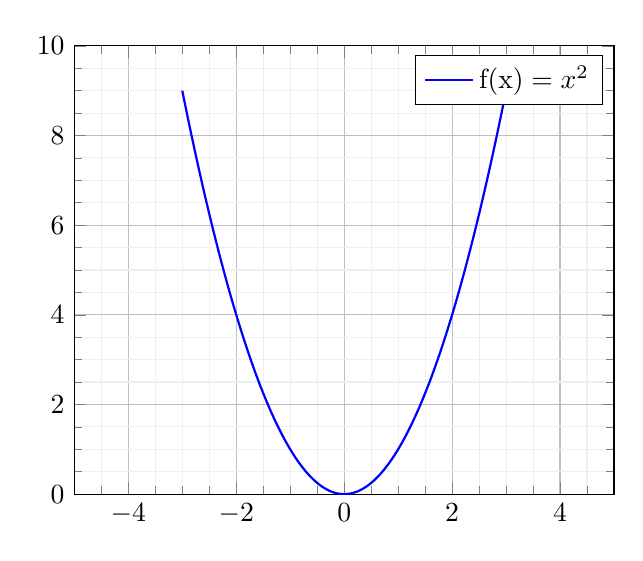
\begin{tikzpicture}

\begin{axis}[
    xmin = -5, xmax = 5,
    ymin = 0, ymax = 10,
    xtick distance = 2,
    ytick distance = 2,
    grid = both,
    minor tick num = 3,
    major grid style = {lightgray},
    minor grid style = {lightgray!25}
    ]
    \addplot[
        domain = -3:3,
        samples = 200,
        smooth,
        thick,
        blue,
    ] {x^2};
    \legend{$\mathrm{ f(x) } = x^2$}
\end{axis}

\end{tikzpicture}